\begin{frame}
	\frametitle{Adaptive Sampling: Theory}
	 \begin{columns}[onlytextwidth,T]
      \column{\dimexpr\linewidth-6cm-5mm}
        
        Adaptive sampling takes advantage of surrogate information content \textit{during training} to reduce sample quantity.\newline
        
        We developed a technique which is novel in the literature:
        \begin{itemize}
        \item Construct surrogate quality distribution by nearest- neighbour interpolation.
        \item Draw candidate samples by quality using MCMC.
        \item Include samples with high crowding distance.
        \item Repeat!
        \end{itemize}
      \column{6cm}
      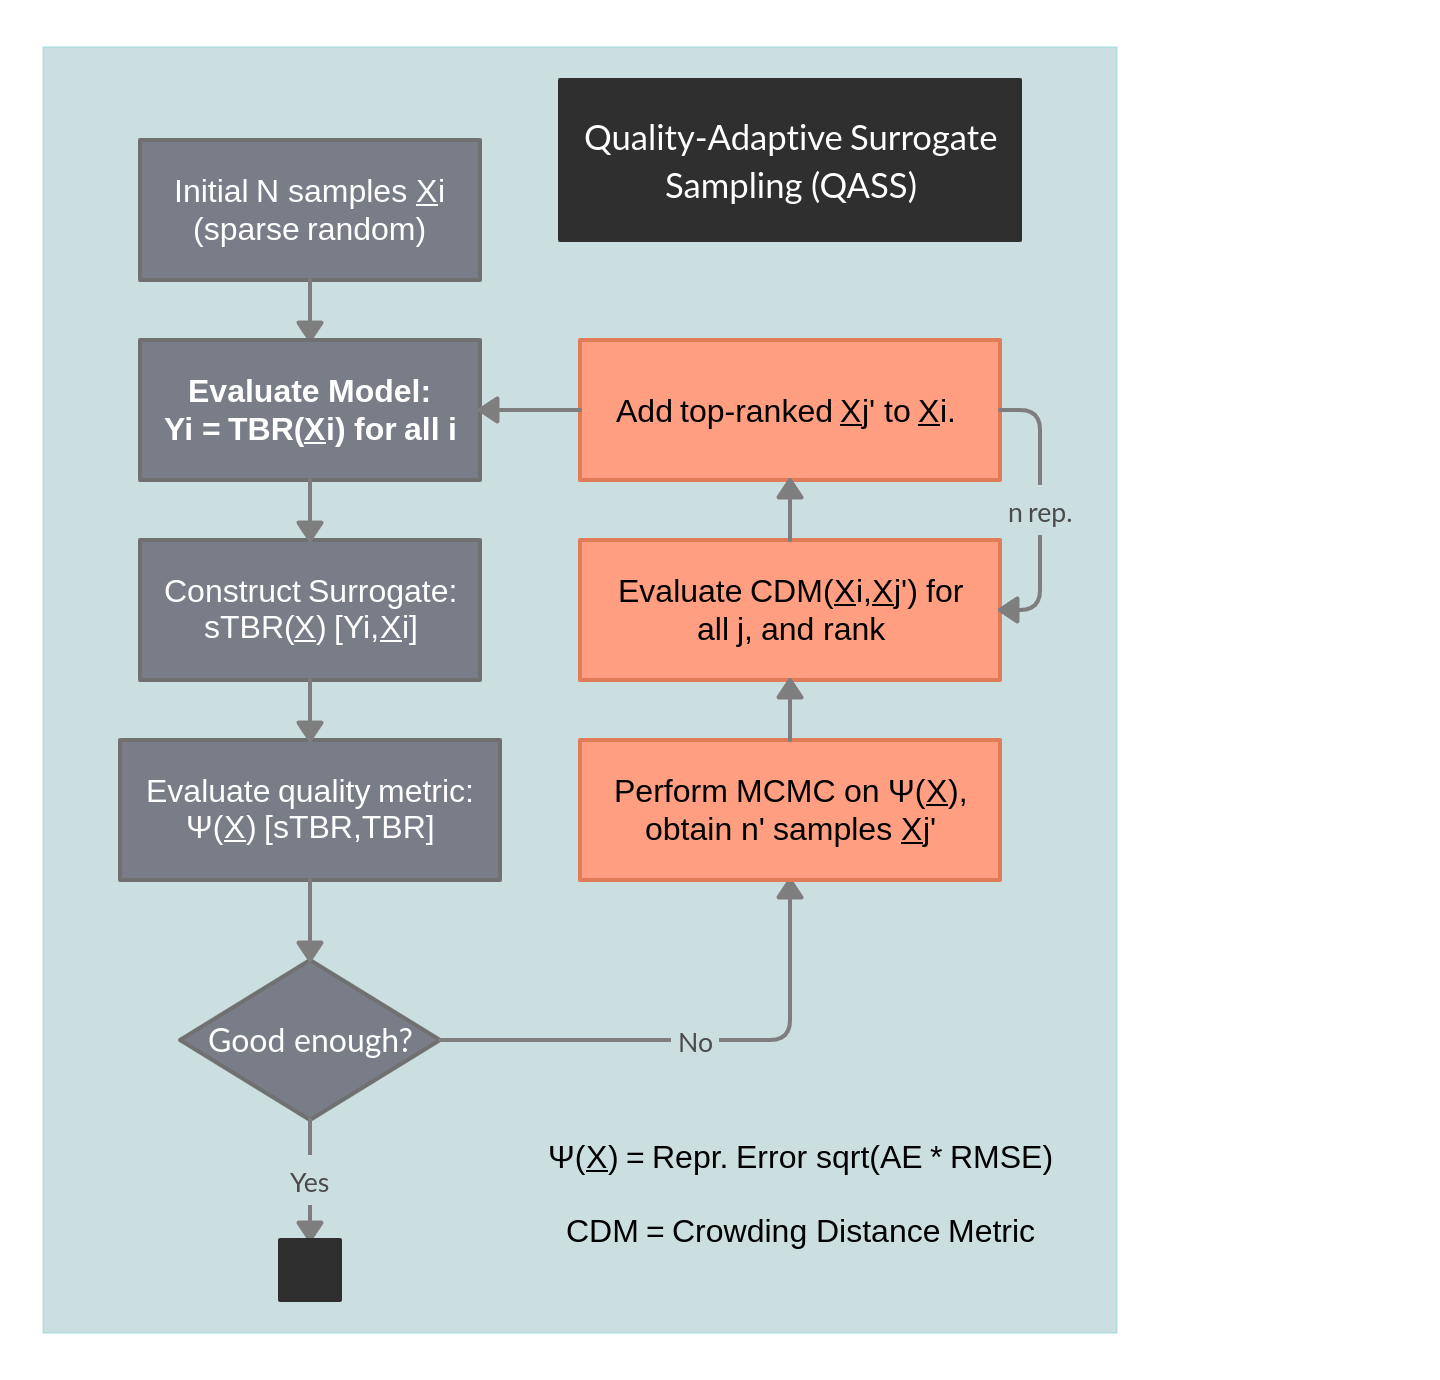
\includegraphics[width=8cm]{qassplan}

    \end{columns}
\end{frame}

\begin{frame}
	\frametitle{Application on Toy Theory}
	Toy functional TBR theory with wavenumber n, and similar ANN performance to Paramak:
	\begin{align*}
		\text{TBR} = \frac{1}{|C|}\sum_{i \in C} \left[1 + \sin(2\pi n (x_i - 1/2)) \right]
	\end{align*}

	\vspace{1em}

	\begin{columns}[T]
		\column{0.5\paperwidth}
		\vspace{0.5em}
		Evaluation performed both on the adaptively-sampled dataset and on a baseline uniform-random dataset.\newline

		An baseline scheme with incremental but uniform-random samples used as a placebo comparison.


		\column{0.4\paperwidth}
		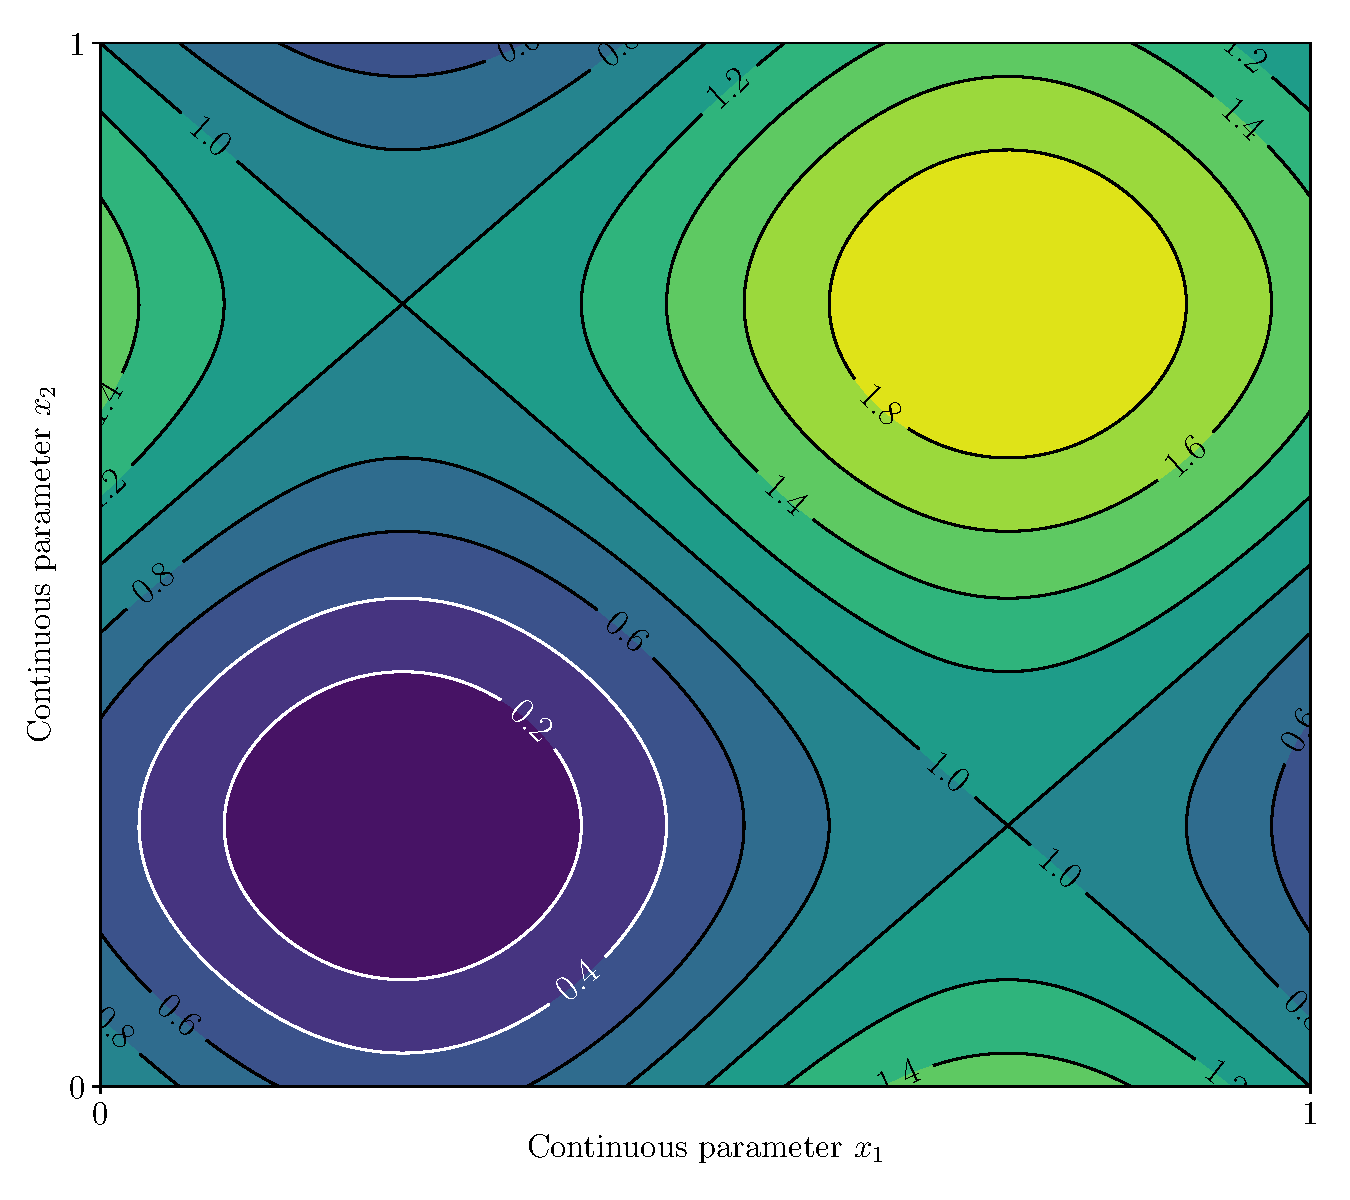
\includegraphics[width=0.4\paperwidth]{sintoy}

	\end{columns}
\end{frame}

\begin{frame}
    \frametitle{Adaptive Sampling: Results}
    
    \begin{center}
    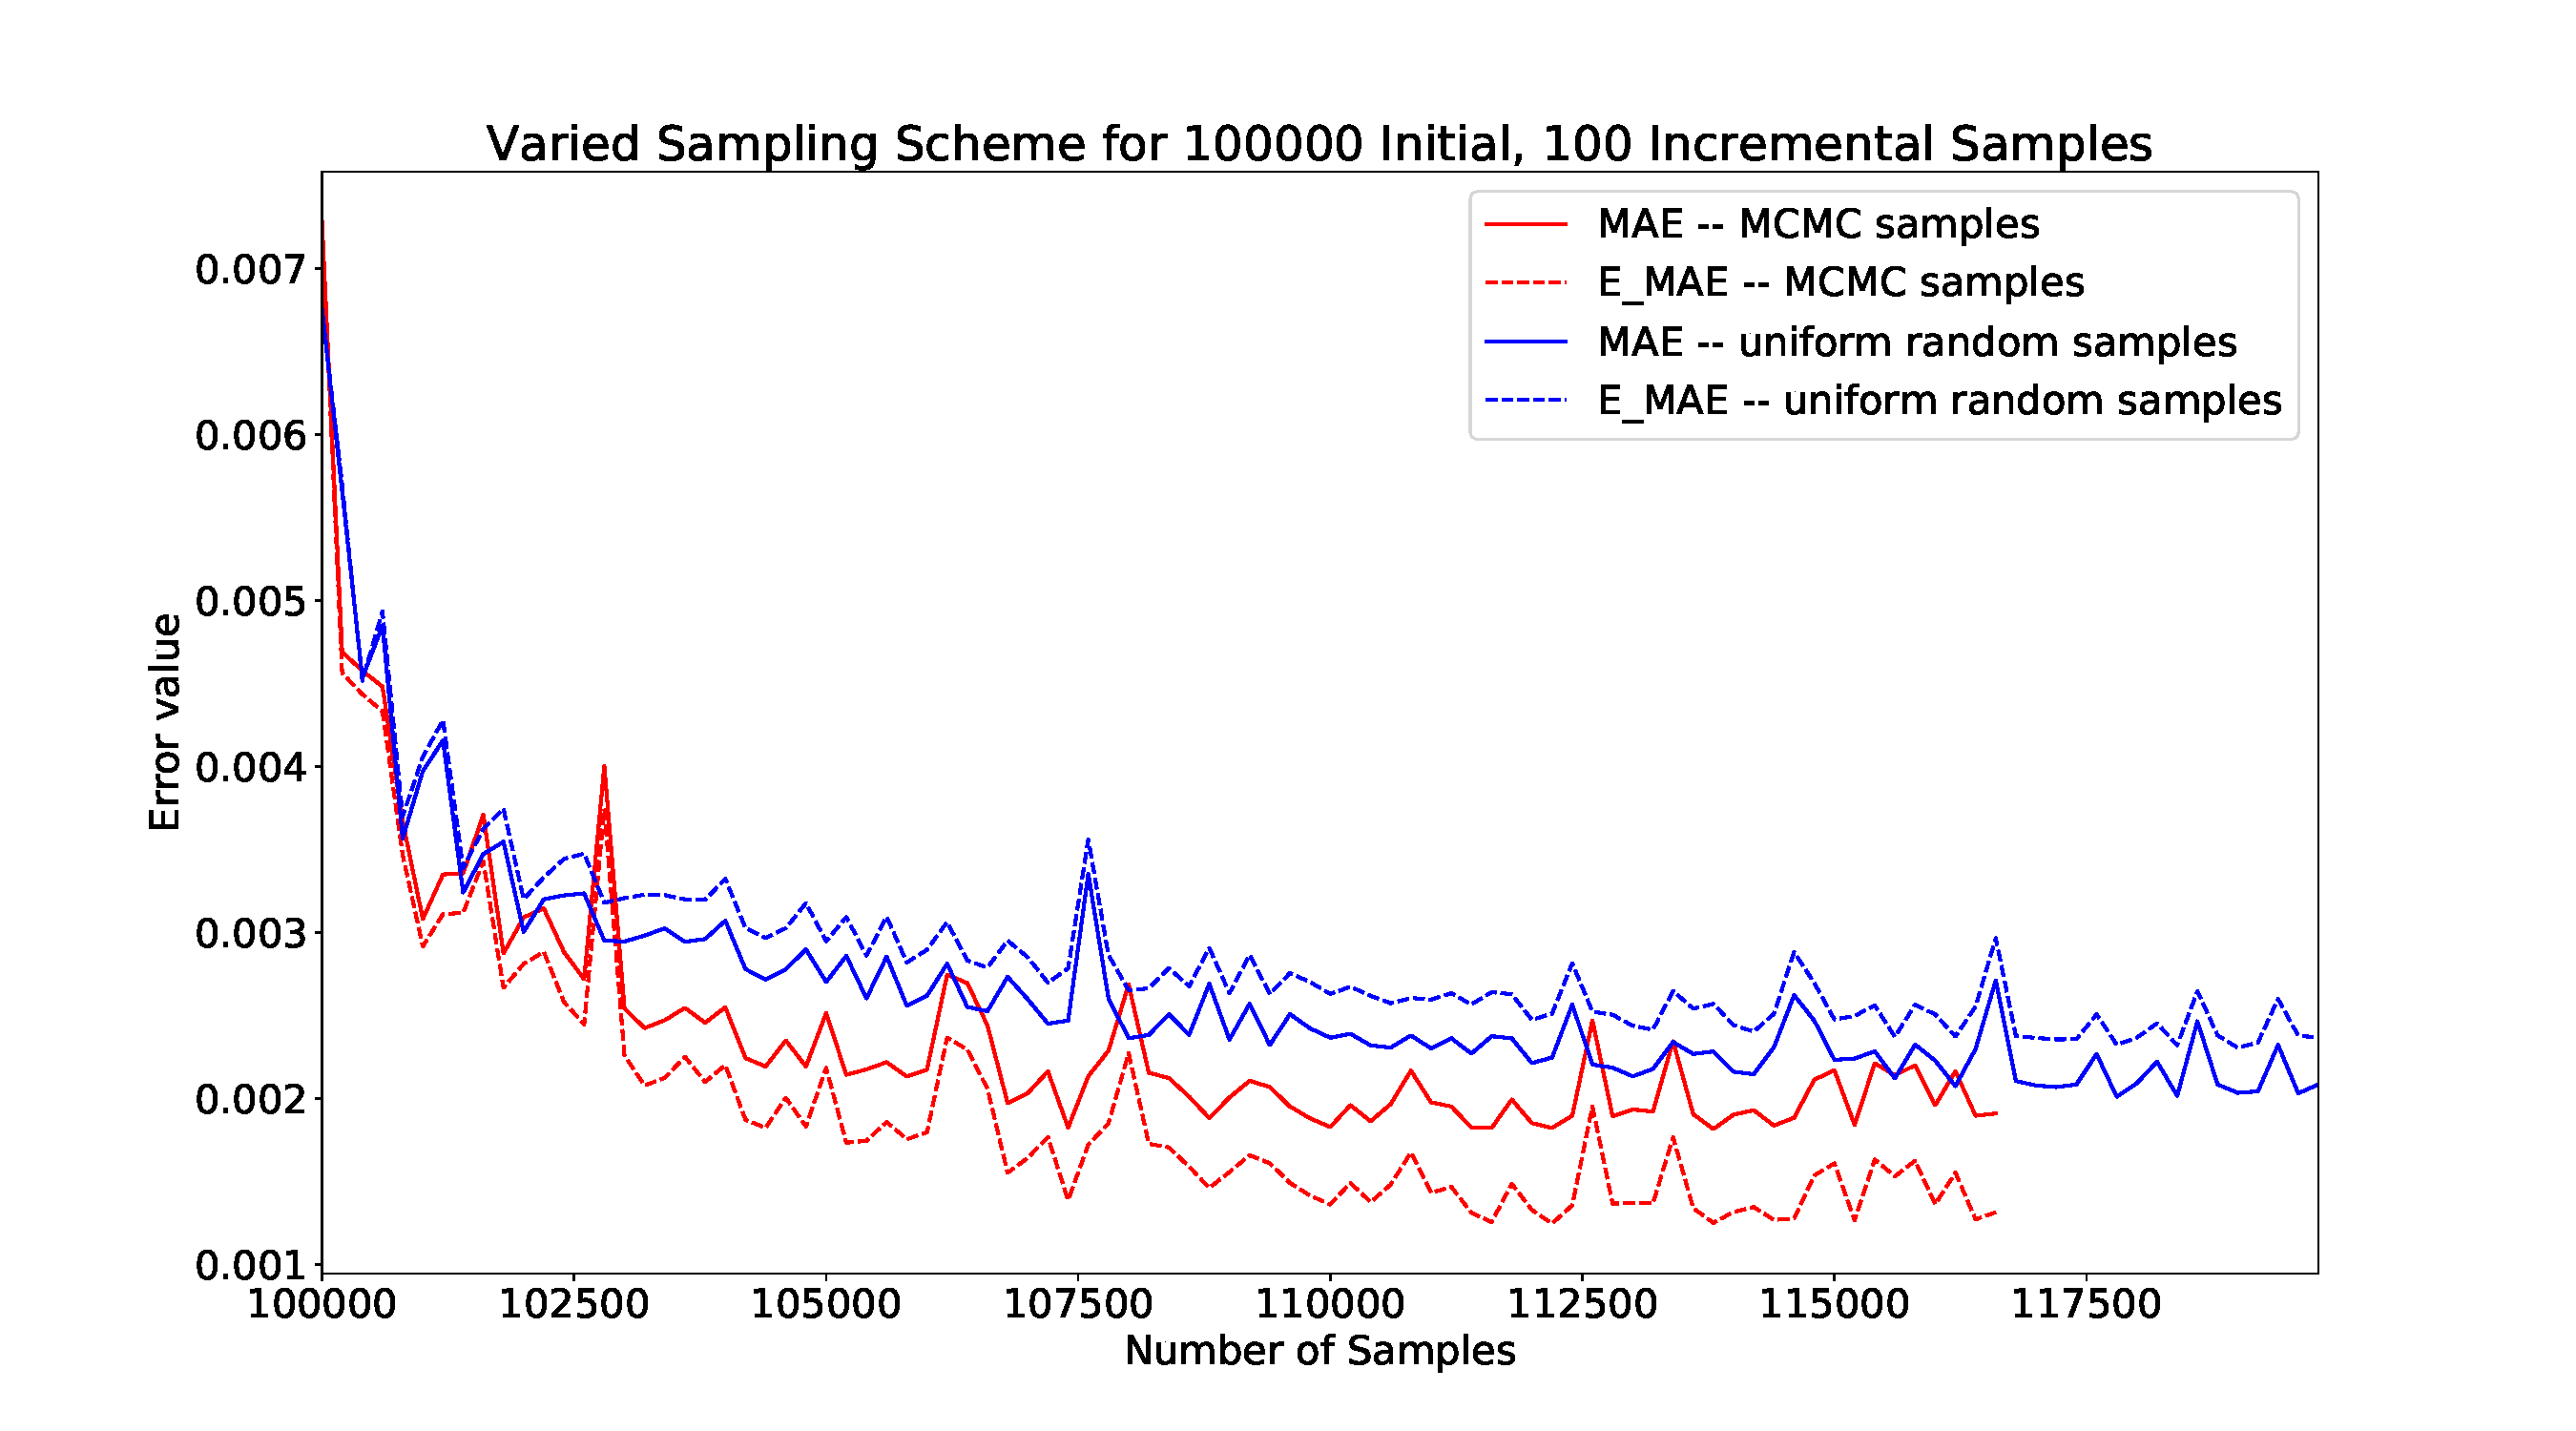
\includegraphics[width=12cm]{qassresult}
    \end{center}

\end{frame}
